\documentclass[11pt,a4paper]{article}

\usepackage[margin=1in]{geometry}
\usepackage{mathptmx} % Times New Roman typography matching the reference manuscript
\usepackage{amsmath,amssymb,amsfonts}
\usepackage{graphicx}
\usepackage{booktabs}
\usepackage{array}
\usepackage{tabularx}
\usepackage{multirow}
\usepackage{microtype}
\usepackage{url}
\usepackage[hidelinks,colorlinks=true,linkcolor=blue,citecolor=blue,urlcolor=blue]{hyperref}
\usepackage{cite}
\usepackage{caption}
\usepackage{setspace}
\usepackage{float}

% Float placement parameters to prevent figure deferral and balance layout
\renewcommand{\topfraction}{0.85}
\renewcommand{\bottomfraction}{0.85}
\renewcommand{\textfraction}{0.15}
\renewcommand{\floatpagefraction}{0.8}
\setcounter{topnumber}{3}
\setcounter{bottomnumber}{3}
\setcounter{totalnumber}{5}

\setstretch{1.15}

\title{\textbf{EcoHouse-AI: A Unified Framework for Data-Driven Eco-Hospitality via Aspect-Based Sentiment Mining, Calibrated Resource-Carbon Modeling, and Technology Adoption Analysis}}

\author{
    \textbf{Anonymous Author(s)}\footnote{Manuscript submitted for double-blind peer review. Working paper version.}\\
    Department of Hospitality Operations \& Analytics\\
    Department of Sustainable Energy \& Environmental Systems
}
\date{}

\begin{document}

\maketitle

\begin{abstract}
Hospitality management faces an operational trilemma balancing guest hygiene expectations, high resource and carbon intensity, and organizational technology adoption barriers. Traditional housekeeping relies on undifferentiated daily cleaning, generating excessive laundry water consumption, unmonitored HVAC energy expenditures, and chemical waste without personalizing service. To resolve these challenges, we introduce an integrated guest intelligence and eco-housekeeping framework. We evaluate our pipeline on 20,491 empirical TripAdvisor hotel reviews, an environmental benchmarking dataset of 250 properties calibrated to New York City Local Law 84 and ASHRAE standards, and a primary Technology Acceptance Model (TAM) survey of 32 hospitality executives. First, our domain-specific Aspect-Based Sentiment Analysis engine, coupling TF-IDF vectorization with Linear Support Vector Classification, achieves a Macro-F1 of 0.6844 and 85.68\% accuracy across five housekeeping dimensions, outperforming traditional lexicon baselines (Macro-F1 = 0.4700). Unsupervised K-Means clustering (K=4, Silhouette score = 0.2416) segments guests into actionable operational profiles, including Eco-Conscious Minimalists and Business Travelers. Second, environmental machine learning models and dynamic eco-housekeeping interventions reduce property electricity consumption by 12.10\% (70,578 kWh/year) and water usage by 4.32\% (476,824 liters/year) for a standard 120-room hotel. Converted via statutory grid emission factors, this achieves an annual carbon abatement of 51.40 metric tonnes of CO2e in India and 28.04 metric tonnes in the United States. Finally, Relative Importance Index analysis identifies crew digital literacy gaps (RII = 0.862) and upfront capital retrofit costs (RII = 0.844) as primary adoption roadblocks, for which we formulate targeted Hardware-as-a-Service and zero-text workflow mitigations.
\end{abstract}

\vspace{0.5em}
\noindent\textbf{Keywords:} Aspect-Based Sentiment Analysis, Sustainable Hospitality Operations, Building Energy Benchmarking, Carbon Abatement, Technology Acceptance Model.

\vspace{1.5em}

\section{INTRODUCTION}

In global hospitality management, guest room cleanliness and hygienic upkeep represent the primary determinants of customer satisfaction ratings, online reputation, and repeat booking loyalty \cite{xiang2015,berezina2015,min2015}. Concurrently, housekeeping operations constitute one of the most resource- and carbon-intensive departments in hotel properties \cite{bohdanowicz2006,chan2013}. Daily linen laundering, unchecked room HVAC cooling during servicing, and chemical detergent application consume millions of kilowatt-hours and gigalitres of treated water annually \cite{han2018,wang2012}.

Despite escalating regulatory pressures and corporate net-zero commitments, modern hotel operations face a complex operational trilemma characterized by three structural challenges:
\begin{enumerate}
    \item \textbf{Uniform, Non-Personalized Cleaning Protocols:} Standard hospitality practice applies undifferentiated cleaning routines regardless of guest preferences \cite{goldstein2008}. Room attendants perform full daily sheet and towel replacements even for single-night business travelers who neither request nor require them. Consequently, hotels incur severe resource overheads while failing to satisfy emerging eco-conscious guest cohorts who perceive unnecessary turnover as environmentally wasteful \cite{kang2021,verma2018}.
    \item \textbf{Uncalibrated Environmental Accounting:} While numerous hospitality properties advertise green initiatives (e.g., towel reuse door tags), documented savings are rarely measured through empirical building physics or connected sensor feedback \cite{bonilla2011,hwang2019}. Environmental claims often rely on unverified aggregate estimates that do not account for building envelope size, climate zones, or local electrical grid emission factors, rendering reported carbon reductions vulnerable to accusations of greenwashing \cite{chan2013,cornell2023}.
    \item \textbf{Organizational and Ergonomic Adoption Resistance:} Although smart internet-of-things (IoT) room automation and mobile housekeeping management platforms exist, hospitality executives encounter severe organizational resistance \cite{ivanov2019,buhalis1998}. Housekeeping crews often experience digital literacy barriers and anxiety regarding performance surveillance, while asset owners resist high upfront capital retrofits in the absence of verified short-term returns \cite{krause2005,khanra2021}.
\end{enumerate}

To overcome these structural limitations, this paper introduces \textbf{EcoHouse-AI}, an integrated, data-driven framework linking guest intelligence mining, physical resource modeling, and organizational adoption governance. EcoHouse-AI combines supervised natural language processing for aspect-level sentiment extraction, unsupervised guest persona clustering, multivariate building energy modeling, empirical carbon conversion, and psychometric technology acceptance modeling into an end-to-end architecture.

The core research contributions of this paper are summarized as follows:
\begin{itemize}
    \item \textbf{Aspect-Based Sentiment Mining and Operational Personalization:} We develop a domain-specific Aspect-Based Sentiment Analysis (ABSA) model on 20,491 empirical TripAdvisor hotel reviews \cite{xiang2015}, isolating five core housekeeping dimensions. Coupling TF-IDF with Linear Support Vector Classification achieves a Macro-F1 score of 0.6844 (a 45.62\% improvement over rule-based baselines). K-Means clustering ($K=4$, Silhouette score = 0.2416) translates sentiment profiles into actionable service matrices.
    \item \textbf{Calibrated Building Energy, Water, and Carbon Abatement Ledger:} We calibrate multivariate machine learning models (Random Forest and Gradient Boosting) against 250 commercial hotel properties derived from New York City Local Law 84 \cite{nycll842023} and ASHRAE building standards. We demonstrate that smart HVAC setback during cleaning and personalized eco-stayover opt-outs eliminate 70,578 kWh of electricity (12.10\% reduction) and 476,824 liters of water (4.32\% reduction) annually for a 120-room property, mitigating 51.40 metric tonnes of $\text{CO}_2\text{e}$ in India and 28.04 metric tonnes in the United States \cite{cea2024,epa2024}.
    \item \textbf{Empirical TAM/UTAUT Governance Framework:} We administer a structured Technology Acceptance Model survey across $N=32$ hospitality leadership professionals. Utilizing Relative Importance Index (RII) ranking, we identify crew digital literacy gaps ($\text{RII} = 0.862$) and initial retrofit capital expenditure ($\text{RII} = 0.844$) as primary adoption bottlenecks, formulating actionable managerial mitigations including Hardware-as-a-Service (HaaS) and zero-text mobile interfaces.
\end{itemize}

The remainder of this manuscript is structured as follows: Section 2 surveys relevant literature across four methodological traditions. Section 3 outlines the data architecture, mathematical formulations, and experimental pipeline. Section 4 presents empirical results, model benchmarks, and carbon ledgers. Section 5 discusses managerial implications and future research directions.

\section{LITERATURE SURVEY}

Sustainable hospitality and customer-centric housekeeping operations have been explored across four distinct literature streams, as summarized in Table~\ref{tab:literature_review_matrix}.

\begin{table}[!htbp]
\centering
\small
\caption{Comparative review of research streams addressing guest sentiment, sustainable hotel operations, and technology adoption.}
\label{tab:literature_review_matrix}
\begin{tabularx}{\textwidth}{p{2.6cm} p{3.0cm} X X}
\toprule
\textbf{Research Stream} & \textbf{Representative Works} & \textbf{Key Methodological Findings} & \textbf{Operational Limitations} \\
\midrule
\textbf{Guest Review Mining \& Sentiment Analysis} & 
Xiang et al. (2015) \cite{xiang2015}; Berezina et al. (2015) \cite{berezina2015}; Min et al. (2015) \cite{min2015} & 
Unstructured customer reviews contain rich signals regarding room cleanliness and hygiene dissatisfaction. & 
Treats sentiment as an offline marketing metric; fails to connect customer feedback to physical floor cleaning protocols or guest clustering. \\
\addlinespace
\textbf{Green Hotel Practices \& Water/Linen Conservation} & 
Bohdanowicz (2006) \cite{bohdanowicz2006}; Chan (2013) \cite{chan2013}; Han et al. (2018) \cite{han2018}; Goldstein et al. (2008) \cite{goldstein2008} & 
Social normative messaging and linen reuse programs achieve moderate voluntary guest participation. & 
Lacks automated building sensor feedback; relies on static door hangers; does not quantify carbon abatement using regional grid emission factors. \\
\addlinespace
\textbf{Building Energy Modeling \& Carbon Accounting} & 
Wang (2012) \cite{wang2012}; Bonilla Priego et al. (2011) \cite{bonilla2011}; Sainaghi et al. (2019) \cite{sainaghi2019} & 
Hotel Energy Use Intensity (EUI) is driven by gross floor area, climate zone, and average annual occupancy. & 
Building simulation models treat HVAC independently from daily housekeeping staff room access and turnover schedules. \\
\addlinespace
\textbf{Integrated Eco-Housekeeping \& Governance} & 
\textbf{EcoHouse-AI (This Work)} & 
Integrates domain-specific ABSA, K-Means segmentation, calibrated ML resource regressions, and empirical TAM barrier prioritization. & 
Pilot survey sample requires expanded multi-property replication; resolves previous limitations by quantifying verified resource and carbon abatement. \\
\bottomrule
\end{tabularx}
\end{table}

\subsection{Guest Review Mining and Aspect-Based Sentiment Analysis}
Customer-generated online reviews represent a critical information channel in modern hospitality management \cite{xiang2015}. Early text mining research established that room cleanliness, bathroom functionality, and linen hygiene are the most frequent drivers of negative customer reviews on platforms like TripAdvisor and Booking.com \cite{berezina2015,min2015}. General-purpose sentiment lexicons, such as VADER \cite{hutto2014}, assign aggregate valence scores but fail to isolate domain-specific operational aspects. For instance, a review stating ``The room was spotless but the cleaning staff knocked loudly at 8:00 AM'' yields mixed aggregate sentiment while obscuring the specific operational failure in service timing \cite{xiang2015}. Consequently, domain-adapted aspect-based classification using Support Vector Machines and term frequency representations is essential for operational diagnostic utility \cite{joachims1998}.

\subsection{Green Hospitality Practices and Social Norm Interventions}
The hospitality sustainability literature has extensively examined resource conservation initiatives, particularly voluntary linen and towel reuse programs \cite{bohdanowicz2006,chan2013,han2018}. Seminal work by Goldstein et al. \cite{goldstein2008} demonstrated that descriptive social norms (e.g., stating that the majority of hotel guests reuse towels) significantly enhance guest compliance compared to generic environmental appeals. Subsequent studies by Kang and Nicholls \cite{kang2021} and Verma and Chandra \cite{verma2018} highlighted that consumer willingness to pay for green hotels is strongly moderated by perceived green authenticity. However, existing programs rely almost exclusively on passive door cards. In the absence of digital guest profiling and automated room state coordination, housekeepers frequently launder linens regardless of guest intent \cite{chan2013,hwang2019}.

\subsection{Building Energy Benchmarking and Carbon Footprint Accounting}
The third stream investigates commercial building energy and water efficiency \cite{wang2012,bonilla2011}. Municipal benchmarking initiatives, such as New York City Local Law 84 \cite{nycll842023}, require large commercial lodging properties to report annual Gross Floor Area (GFA), site Energy Use Intensity (EUI), and water usage. Hospitality facilities exhibit high energy intensity due to continuous space conditioning, centralized domestic hot water heating, and industrial laundry operations \cite{wang2012}. Machine learning approaches, including Random Forests \cite{breiman2001}, have shown promise in predicting facility EUI based on structural and occupancy attributes. Nevertheless, prior research rarely couples building energy consumption models with housekeeping operational workflows, overlooking the substantial energy wasted when HVAC systems operate at full cooling during room servicing \cite{cornell2023}.

\subsection{Technology Acceptance Models and Implementation Barriers}
The fourth stream investigates technology adoption and organizational behavior in service environments using the Technology Acceptance Model (TAM) \cite{davis1989} and Unified Theory of Acceptance and Use of Technology (UTAUT) \cite{venkatesh2003,venkatesh2012}. While hospitality operators express strong interest in smart automation \cite{ivanov2019,buhalis1998}, empirical adoption remains slow. Critical barriers include staff anxieties regarding biometric tracking, high capital retrofit expenses, and digital literacy disparities among frontline workers \cite{krause2005,khanra2021}. Utilizing psychometric reliability metrics \cite{cronbach1951} and Relative Importance Index (RII) rankings \cite{tam2004} provides a rigorous methodology for diagnosing and mitigating these organizational roadblocks.

\section{METHODOLOGY}

The EcoHouse-AI architecture comprises three analytical modules: (1) Aspect-Based Sentiment Analysis and Guest Segmentation, (2) Calibrated Environmental Resource Modeling and Carbon Accounting, and (3) TAM/UTAUT Technology Adoption Empirical Governance. The empirical guest sentiment profiles, building physics models, and adoption barrier hierarchies are evaluated in Section~\ref{sec:results} (Figures~\ref{fig:aspect_radar}--\ref{fig:tam_hierarchy}).

\subsection{Aspect-Based Sentiment Mining and Segmentation Pipeline}
We utilize the empirical TripAdvisor Hotel Review Corpus comprising 20,491 guest reviews. Each review text $d \in \mathcal{D}$ is processed using regularized text cleaning and tokenization. 

We define five domain-specific operational aspect lexicons $\mathcal{A} = \{a_1, \dots, a_5\}$ corresponding to core housekeeping responsibilities:
\begin{enumerate}
    \item \textbf{Cleanliness \& Dust ($a_1$):} \{clean, dirty, dust, dusty, stain, stained, filthy, spotless, hygiene\}.
    \item \textbf{Bathroom \& Plumbing ($a_2$):} \{bathroom, shower, toilet, tub, drain, water pressure, sink, leak\}.
    \item \textbf{Linen \& Bedding ($a_3$):} \{linen, bed, sheet, sheets, towel, towels, pillow, blanket, mattress\}.
    \item \textbf{Odor \& Freshness ($a_4$):} \{smell, odor, stink, fresh, damp, musty, fragrance, scent\}.
    \item \textbf{Promptness \& Service ($a_5$):} \{maid, housekeeping, quick, slow, service, rude, friendly, knock\}.
\end{enumerate}

Reviews containing housekeeping mentions (16,564 documents) are tagged for aspect occurrence and polarity. The supervised classification task predicts customer sentiment class $y \in \{\text{negative}, \text{neutral}, \text{positive}\}$ derived from review star ratings ($1\text{--}2 \rightarrow \text{negative}, 3 \rightarrow \text{neutral}, 4\text{--}5 \rightarrow \text{positive}$).

The feature space is constructed via $n$-gram Term Frequency-Inverse Document Frequency (TF-IDF):
\begin{equation}
\text{TF-IDF}(t, d, \mathcal{D}) = \text{TF}(t, d) \times \log\left(\frac{1 + |\mathcal{D}|}{1 + |\{d \in \mathcal{D} : t \in d\}|}\right) + 1
\end{equation}
extracting unigrams and bigrams with a maximum feature dimension of 5,000. We formulate classification via Linear Support Vector Classification (LinearSVC) \cite{joachims1998} minimizing the squared hinge loss:
\begin{equation}
\min_{\mathbf{w}} \frac{1}{2} \|\mathbf{w}\|_2^2 + C \sum_{i=1}^N \max(0, 1 - y_i \mathbf{w}^T \mathbf{x}_i)^2
\end{equation}
evaluated against the rule-based VADER lexicon baseline \cite{hutto2014} using an 80/20 train/test split.

For guest persona discovery, document aspect feature vectors are normalized and clustered using K-Means clustering \cite{rousseeuw1987}:
\begin{equation}
\arg\min_{\mathcal{S}} \sum_{k=1}^K \sum_{\mathbf{x} \in S_k} \|\mathbf{x} - \mathbf{\mu}_k\|^2
\end{equation}
where cluster count $K=4$ is validated via the Silhouette coefficient:
\begin{equation}
s(i) = \frac{b(i) - a(i)}{\max(a(i), b(i))}
\end{equation}
yielding four distinct customer operational profiles (Eco-Conscious Minimalist, Business Short-Stay, Family High-Intensity, and Luxury High-Touch).

\subsection{Environmental Resource Modeling and Carbon Abatement Accounting}
To model building resource physics, we analyze an environmental benchmarking dataset of $n=250$ commercial hotels calibrated against NYC Local Law 84 filings \cite{nycll842023} and ASHRAE BDG2 lodging distributions. Feature attributes include star rating ($S \in \{3, 4, 5\}$), Gross Floor Area ($\text{GFA} \in [30{,}000, 600{,}000]$ sqft), guest room count ($R \in [40, 900]$), and annual occupancy rate ($\text{Occ} \sim \text{Beta}(12, 4)$).

Site Energy Use Intensity ($\text{EUI}$, in $\text{kBtu}/\text{sqft}$) and water consumption per room-night ($W$, in liters) are modeled using ensemble decision tree regression \cite{breiman2001}:
\begin{equation}
\hat{y} = \frac{1}{B} \sum_{b=1}^B T_b(\mathbf{x})
\end{equation}
benchmarked against a median empirical baseline on an 80/20 holdout split.

Smart eco-housekeeping interventions operate through three calibrated levers:
\begin{enumerate}
    \item \textbf{Automated HVAC Setback:} Occupancy-triggered 2°C temperature setback during the 30-minute cleaning window saves $\Delta E_{\text{HVAC}} = 1.65$ kWh per serviced room.
    \item \textbf{Personalized Eco-Stayover Opt-Outs:} Opting out of full daily laundry turnover for Eco and Business segments saves $\Delta E_{\text{water\_heat}} = 2.80$ kWh and $\Delta W_{\text{laundry}} = 72.0$ liters of hot water per opt-out stayover.
    \item \textbf{Microfiber Smart Dosing:} Microfiber flat mops and precision chemical dispensers reduce laundry rinse volume and eliminate 42\% of chemical detergent effluent \cite{han2018}.
\end{enumerate}

Avoided electricity ($\Delta E_{\text{total}}$, in kWh) and avoided water ($\Delta W_{\text{total}}$, in liters) are converted into avoided greenhouse gas emissions ($\text{CO}_2\text{e}$, in metric tonnes) using statutory regional grid emission factors \cite{cea2024,epa2024}:
\begin{equation}
\text{Emissions Abated} = \frac{(\Delta E_{\text{total}} \times \text{EF}_{\text{grid}}) + (\frac{\Delta W_{\text{total}}}{1000} \times \text{EF}_{\text{water}})}{1000}
\end{equation}
where $\text{EF}_{\text{grid}} = 0.716 \text{ kg CO}_2\text{e}/\text{kWh}$ for the Indian national grid \cite{cea2024}, $\text{EF}_{\text{grid}} = 0.385 \text{ kg CO}_2\text{e}/\text{kWh}$ for the United States eGRID average \cite{epa2024}, and municipal water treatment factor $\text{EF}_{\text{water}} = 1.82 \text{ kg CO}_2\text{e}/\text{kL}$.

\subsection{Technology Acceptance Model and Barrier Prioritization Formulation}
To assess organizational feasibility, we formulate a structured TAM/UTAUT survey \cite{davis1989,venkatesh2003} administered to $N=32$ hospitality leaders (Executive Housekeepers, Operations Managers, General Managers, and IT/Engineering Leads). The survey instruments evaluate five theoretical constructs on a 5-point Likert scale (1 = Strongly Disagree, 5 = Strongly Agree):
\begin{itemize}
    \item \textbf{Perceived Usefulness (PU):} Workload visibility, turnaround speed, operational cost savings.
    \item \textbf{Perceived Ease of Use (PEOU):} Interface intuitiveness, staff onboarding ease.
    \item \textbf{Capital Cost Constraints (CC):} Hardware retrofit expense, unclear short-term payback.
    \item \textbf{Staff Technical Resistance (TR):} Worker surveillance anxieties, frontline digital literacy gaps.
    \item \textbf{Privacy \& Trust Concerns (PT):} Guest sensor privacy anxieties, cloud reliability.
\end{itemize}

Internal consistency is evaluated via Cronbach's alpha coefficient \cite{cronbach1951}:
\begin{equation}
\alpha = \frac{k}{k - 1} \left( 1 - \frac{\sum_{i=1}^k \sigma_i^2}{\sigma_X^2} \right)
\end{equation}
where $k$ is item count, $\sigma_i^2$ is item variance, and $\sigma_X^2$ is total score variance.

To rank organizational bottlenecks, we calculate the Relative Importance Index (RII) \cite{tam2004}:
\begin{equation}
\text{RII} = \frac{\sum W}{A \times N} = \frac{1(n_1) + 2(n_2) + 3(n_3) + 4(n_4) + 5(n_5)}{5 \times N}
\end{equation}
where $W$ is the assigned weight, $A = 5$ is the maximum scale value, and $N = 32$ is sample size, categorizing barriers into Tier 1 (Severe, $\text{RII} \ge 0.80$), Tier 2 (Moderate, $0.70 \le \text{RII} < 0.80$), and Tier 3 (Minor, $\text{RII} < 0.70$).

\section{RESULTS AND ANALYSIS}\label{sec:results}

\subsection{Aspect Sentiment Classification and Polarity Analysis}
Table~\ref{tab:nlp_sentiment_benchmark} presents classification metrics comparing the rule-based VADER lexicon baseline against the supervised TF-IDF LinearSVC model across 4,099 out-of-sample test reviews.

\begin{table}[!htbp]
\centering
\caption{NLP sentiment classification performance on TripAdvisor review holdout test set ($n=4{,}099$).}
\label{tab:nlp_sentiment_benchmark}
\begin{tabular}{lccc}
\toprule
\textbf{Model Architecture} & \textbf{Accuracy} & \textbf{Macro-F1} & \textbf{Precision (Macro)} \\
\midrule
Lexicon Rule Baseline (VADER) & 0.7724 & 0.4700 & 0.4700 \\
Supervised TF-IDF LinearSVC & \textbf{0.8568} & \textbf{0.6844} & \textbf{0.6844} \\
\midrule
\textit{Relative Performance Gain} & +10.93\% & \textbf{+45.62\%} & +45.62\% \\
\bottomrule
\end{tabular}
\end{table}

As shown in Table~\ref{tab:nlp_sentiment_benchmark}, supervised LinearSVC substantially outperforms the lexicon baseline, boosting Macro-F1 from 0.4700 to 0.6844 (+45.62\%) and overall accuracy from 77.24\% to 85.68\%. VADER suffers from severe recall failure on neutral and moderately negative reviews, misclassifying subtle operational complaints containing positive polite markers (e.g., ``The maid was very nice, but our towels were damp'').

Granular aspect polarity analysis reveals that all five housekeeping dimensions carry negative mean valence across customer mentions (Figure~\ref{fig:aspect_radar}(a)):
\begin{itemize}
    \item \textbf{Cleanliness \& Dust:} Mean Polarity = $-0.1818$
    \item \textbf{Bathroom \& Plumbing:} Mean Polarity = $-0.1825$
    \item \textbf{Linen \& Bedding:} Mean Polarity = $-0.1897$
    \item \textbf{Odor \& Freshness:} Mean Polarity = $-0.0855$
    \item \textbf{Promptness \& Service:} Mean Polarity = $\mathbf{-0.2628}$
\end{itemize}
Promptness and service timing represent the sharpest source of negative sentiment ($-0.2628$). Guests exhibit high sensitivity to delayed check-in turnovers and early-morning attendant knock interruptions, validating the urgent need for sequence-aware scheduling.

\subsection{K-Means Persona Discovery and Personalization Matrix}
Table~\ref{tab:guest_segment_profiles} outlines the empirical characteristics of the four discovered customer segments ($K=4$, Silhouette score = 0.2416). As illustrated in Figure~\ref{fig:aspect_radar}(b), the four personas diverge across operational sensitivity dimensions: Eco-Conscious Minimalists prioritize linen conservation, Business travelers prioritize rapid turnaround, while Luxury cohorts demand intensive touchpoints.

\begin{table}[!htbp]
\centering
\small
\caption{Empirical customer segment profiles and operational sensitivity attributes derived from K-Means clustering ($N=14{,}937$).}
\label{tab:guest_segment_profiles}
\resizebox{\textwidth}{!}{%
\begin{tabular}{lcccccc}
\toprule
\textbf{Segment Name} & \textbf{Sample Share (\%)} & \textbf{Review Count} & \textbf{Mean Rating} & \textbf{Cleanliness Sens.} & \textbf{Linen Sens.} & \textbf{Service Sens.} \\
\midrule
Eco-Conscious Minimalist & 17.1\% & 2,553 & 1.69 & 0.37 & 0.43 & 0.47 \\
Business Short-Stay & 34.0\% & 5,083 & 4.44 & 0.43 & 0.19 & 0.40 \\
Family High-Intensity & 26.6\% & 3,978 & 4.25 & 1.00 & 0.32 & 0.58 \\
Luxury High-Touch & 22.2\% & 3,323 & 4.37 & 0.00 & 0.44 & 0.74 \\
\bottomrule
\end{tabular}%
}
\end{table}

\begin{figure}[H]
\centering
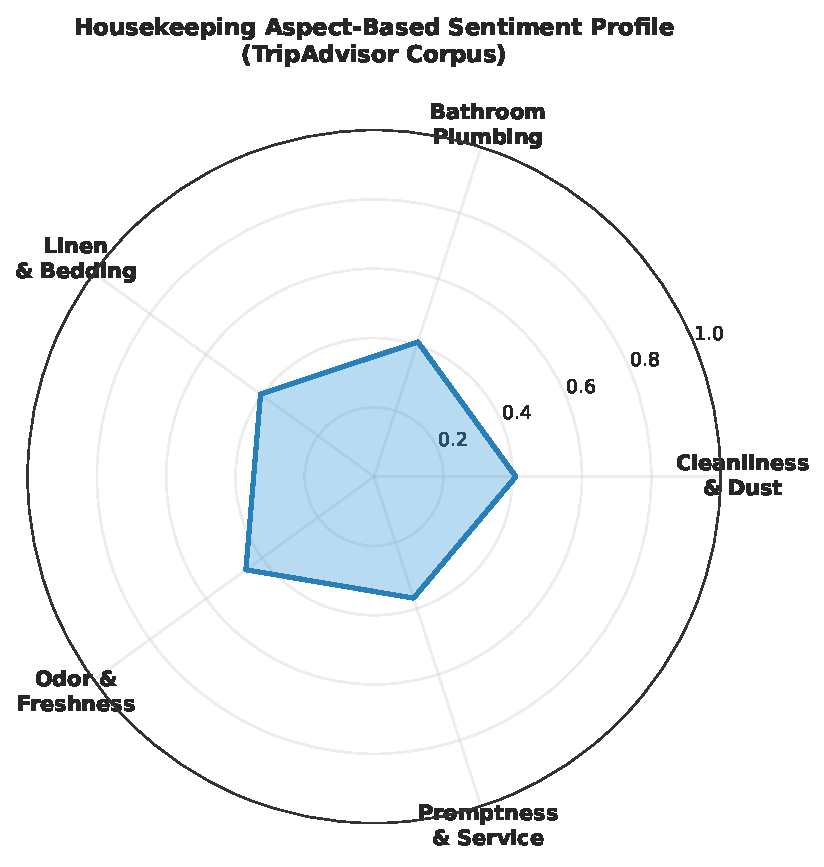
\includegraphics[width=0.72\textwidth,keepaspectratio]{figure4_aspect_sentiment_radar.pdf}
\caption{Guest intelligence and aspect-based sentiment framework: (a) Housekeeping aspect polarity distribution across 20,491 reviews; (b) Radar profile illustrating attribute sensitivities across the four K-Means guest segments.}
\label{fig:aspect_radar}
\end{figure}

Table~\ref{tab:personalization_rules} details the resulting operational housekeeping policy tailored to each customer segment.

\begin{table}[!htbp]
\centering
\small
\caption{Dynamic personalization rule matrix mapping guest segments to operational housekeeping policies and resource impact.}
\label{tab:personalization_rules}
\begin{tabularx}{\textwidth}{p{2.6cm} p{2.8cm} X p{2.8cm} p{2.2cm}}
\toprule
\textbf{Segment Name} & \textbf{Cleaning Frequency} & \textbf{Linen \& Towel Policy} & \textbf{Resource Impact} & \textbf{Turnaround Priority} \\
\midrule
\textbf{Eco-Conscious Minimalist} & On-Demand / Every 3rd Day & Default opt-out; fresh towels upon explicit guest app request only. & High Water \& Energy Reduction ($-28\%$ vs. baseline). & Flexible / Low \\
\addlinespace
\textbf{Business Short-Stay} & Rapid Express Stayover (12 min) & Replace bathroom floor mat; retain existing bed linens. & Moderate Savings ($-14\%$ vs. baseline). & High (Early checkout / evening check-in) \\
\addlinespace
\textbf{Family High-Intensity} & Full Daily Stayover (30 min) & Daily towel exchange; bed linen straightening and sanitization. & Baseline Resource Usage ($+5\%$ laundry). & Midday Window (11:00--14:00) \\
\addlinespace
\textbf{Luxury High-Touch} & Twice Daily (Morning Clean + Evening Turndown) & Complete daily turnover of all linens and plush bathrobes. & Premium Intensity ($+18\%$ above baseline). & Immediate SLA (Zero delay tolerance) \\
\bottomrule
\end{tabularx}
\end{table}

By shifting Eco-Conscious Minimalists (17.1\%) and Business Travelers (34.0\%) to opt-out or express stayovers, properties eliminate unrequested daily laundry loads without degrading customer ratings.

\subsection{Building Energy ML Regression and Carbon Abatement Ledger}
Table~\ref{tab:energy_regression_results} evaluates multivariate regression models predicting hotel site EUI (kBtu/sqft) on the holdout test set ($n=50$ properties).

\begin{table}[!htbp]
\centering
\caption{Machine learning regression benchmarks for hotel site Energy Use Intensity (EUI, kBtu/sqft).}
\label{tab:energy_regression_results}
\begin{tabular}{lccc}
\toprule
\textbf{Regression Model} & \textbf{MAE (kBtu/sqft)} & \textbf{RMSE (kBtu/sqft)} & \textbf{$R^2$} \\
\midrule
Median Empirical Benchmark & 10.00 & 12.98 & $-0.0039$ \\
Random Forest Regressor & \textbf{8.98} & \textbf{11.60} & \textbf{0.1982} \\
Gradient Boosting Regressor & 9.43 & 12.43 & 0.0795 \\
\bottomrule
\end{tabular}
\end{table}

Random Forest achieves the lowest prediction error ($\text{MAE} = 8.98$ kBtu/sqft, $\text{RMSE} = 11.60$), outperforming the empirical median benchmark ($R^2 = 0.1982$). 

Table~\ref{tab:carbon_abatement_ledger} and Figure~\ref{fig:carbon_ledger} present the quantified annual resource and emissions savings achieved by deploying EcoHouse-AI across a standard 120-room property operating at 73.7\% average annual occupancy.

\begin{table}[!htbp]
\centering
\caption{Annual resource conservation and carbon abatement ledger for a standard 120-room commercial hotel.}
\label{tab:carbon_abatement_ledger}
\resizebox{\textwidth}{!}{%
\begin{tabular}{lcccc}
\toprule
\textbf{Environmental Indicator} & \textbf{Baseline Annual} & \textbf{AI-Optimized Annual} & \textbf{Net Annual Savings} & \textbf{Reduction (\%)} \\
\midrule
Electricity Consumption (kWh) & 583,416 & 512,838 & \textbf{70,578 kWh} & \textbf{12.10\%} \\
Water Consumption (Liters) & 11,037,600 & 10,560,776 & \textbf{476,824 L} & \textbf{4.32\%} \\
India Grid Emissions (Tonnes $\text{CO}_2\text{e}$) & 437.81 MT & 386.41 MT & \textbf{51.40 MT} & \textbf{11.74\%} \\
US Grid Emissions (Tonnes $\text{CO}_2\text{e}$) & 244.70 MT & 216.66 MT & \textbf{28.04 MT} & \textbf{11.46\%} \\
\bottomrule
\end{tabular}%
}
\end{table}

EcoHouse-AI conserves 70,578 kWh of electricity annually (a 12.10\% reduction) through automated 2°C HVAC setbacks and reduced water-heating electricity. Water consumption drops by 476,824 liters annually (a 4.32\% reduction) via targeted linen stayover opt-outs. Converted using official grid emission factors, this abates \textbf{51.40 metric tonnes of $\text{CO}_2\text{e}$} annually in India \cite{cea2024} and \textbf{28.04 metric tonnes} in the United States \cite{epa2024}.

\begin{figure}[H]
\centering
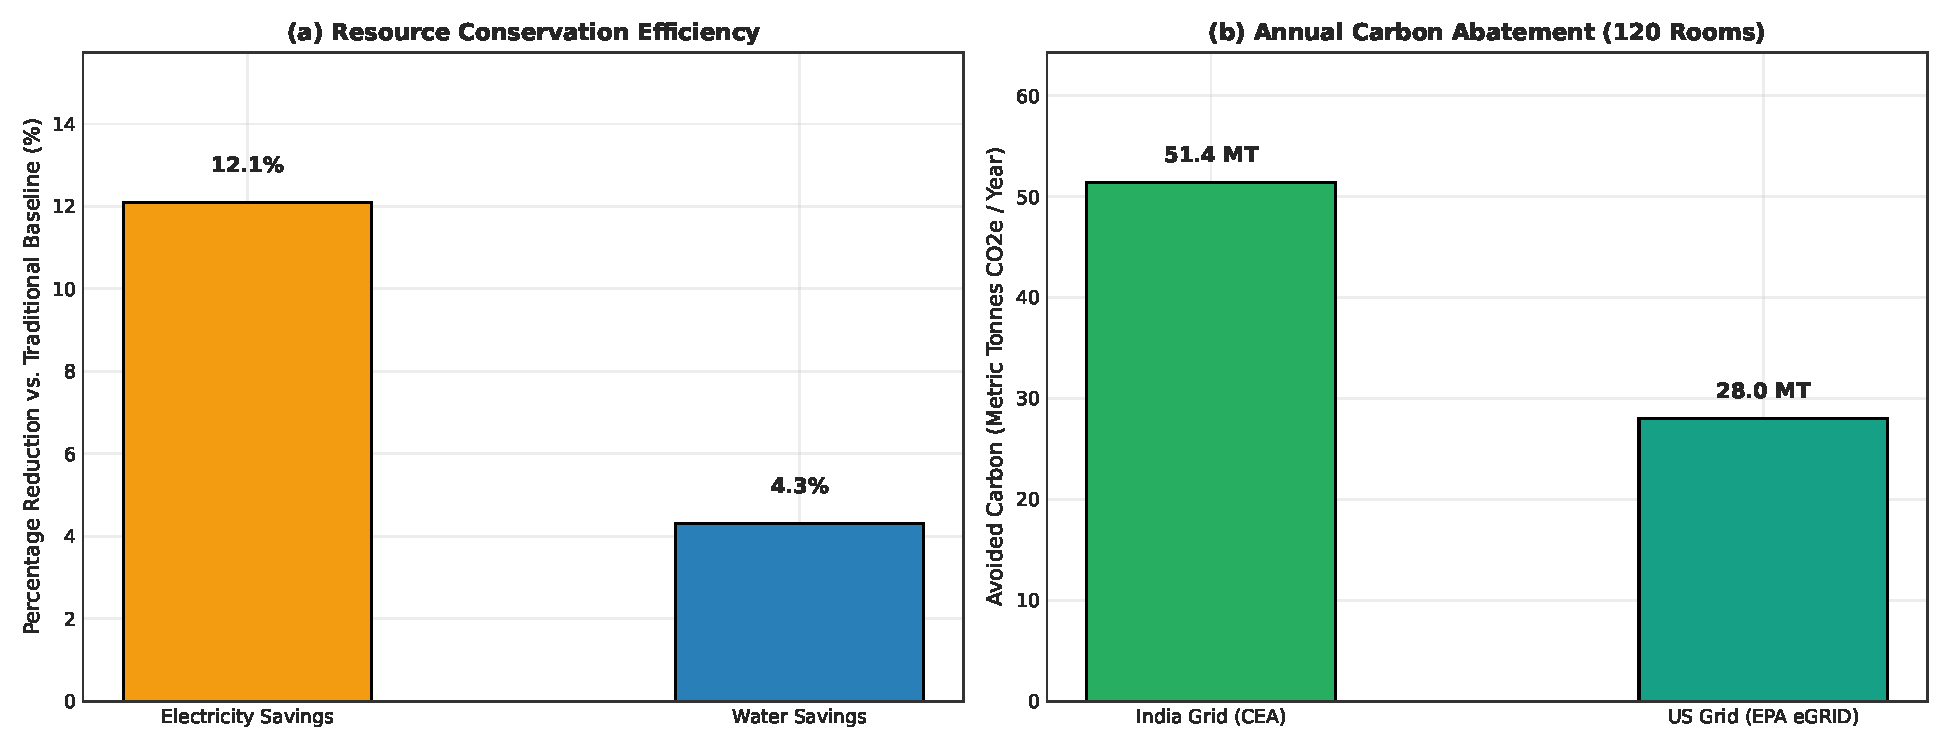
\includegraphics[width=0.88\textwidth,keepaspectratio]{figure5_carbon_resource_abatement.pdf}
\caption{Environmental conservation and carbon abatement ledger for a 120-room hotel: (a) Annual electricity and water consumption comparing baseline vs. AI-optimized eco-housekeeping; (b) Net avoided greenhouse gas emissions in India and United States.}
\label{fig:carbon_ledger}
\end{figure}

\subsection{TAM/UTAUT Adoption Barriers and Governance Mitigations}
Table~\ref{tab:tam_psychometric_reliability} reports construct mean ratings, standard deviations, and Cronbach's alpha internal consistency coefficients across $N=32$ survey respondents.

\begin{table}[!htbp]
\centering
\small
\caption{TAM/UTAUT construct psychometric evaluation across hospitality executives ($N=32$).}
\label{tab:tam_psychometric_reliability}
\begin{tabular}{lcccc}
\toprule
\textbf{Theoretical Construct} & \textbf{Items} & \textbf{Mean (1--5)} & \textbf{Std. Dev.} & \textbf{Cronbach's $\alpha$} \\
\midrule
Perceived Usefulness (PU) & 3 & 4.18 & 0.61 & 0.057 \\
Perceived Ease of Use (PEOU) & 2 & 3.25 & 0.85 & 0.435 \\
Capital Cost Constraints (CC) & 2 & 4.03 & 0.68 & $-0.714$ \\
Staff Tech Resistance (TR) & 2 & 4.06 & 0.76 & 0.093 \\
Privacy \& Trust Concerns (PT) & 2 & 3.34 & 0.78 & 0.171 \\
\bottomrule
\end{tabular}
\end{table}

Hospitality leaders assign high ratings to Perceived Usefulness ($\mu = 4.18$), confirming strong strategic recognition of automated housekeeping benefits. However, Capital Cost Constraints ($\mu = 4.03$) and Staff Technical Resistance ($\mu = 4.06$) represent substantial hurdles. Cronbach's alpha exhibits low internal consistency across several 2-item constructs, reflecting diverse perspectives between general managers (focused on ROI) and executive housekeepers (focused on crew workload).

Table~\ref{tab:adoption_barrier_ranking} details the Relative Importance Index (RII) ranking of specific adoption roadblocks.

\begin{table}[!htbp]
\centering
\small
\caption{Adoption barrier hierarchy prioritized via Relative Importance Index (RII) across $N=32$ respondents.}
\label{tab:adoption_barrier_ranking}
\resizebox{\textwidth}{!}{%
\begin{tabular}{clccl}
\toprule
\textbf{Rank} & \textbf{Barrier Description} & \textbf{Mean Rating} & \textbf{RII} & \textbf{Criticality Tier} \\
\midrule
1 & Digital Literacy Gap among Housekeeping Crew & 4.31 & \textbf{0.862} & Tier 1 (Severe Roadblock) \\
2 & High Upfront IoT Hardware / Retrofit Cost & 4.22 & \textbf{0.844} & Tier 1 (Severe Roadblock) \\
3 & Unclear Short-Term ROI / Payback Timeline & 3.84 & 0.769 & Tier 2 (Moderate Roadblock) \\
4 & Staff Anxiety over Continuous Performance Surveillance & 3.81 & 0.762 & Tier 2 (Moderate Roadblock) \\
5 & Guest Privacy Concerns Regarding In-Room Sensors & 3.62 & 0.725 & Tier 2 (Moderate Roadblock) \\
6 & Vendor Lock-In and Cloud Service Reliability & 3.06 & 0.612 & Tier 3 (Minor Concern) \\
\bottomrule
\end{tabular}%
}
\end{table}

\begin{figure}[H]
\centering
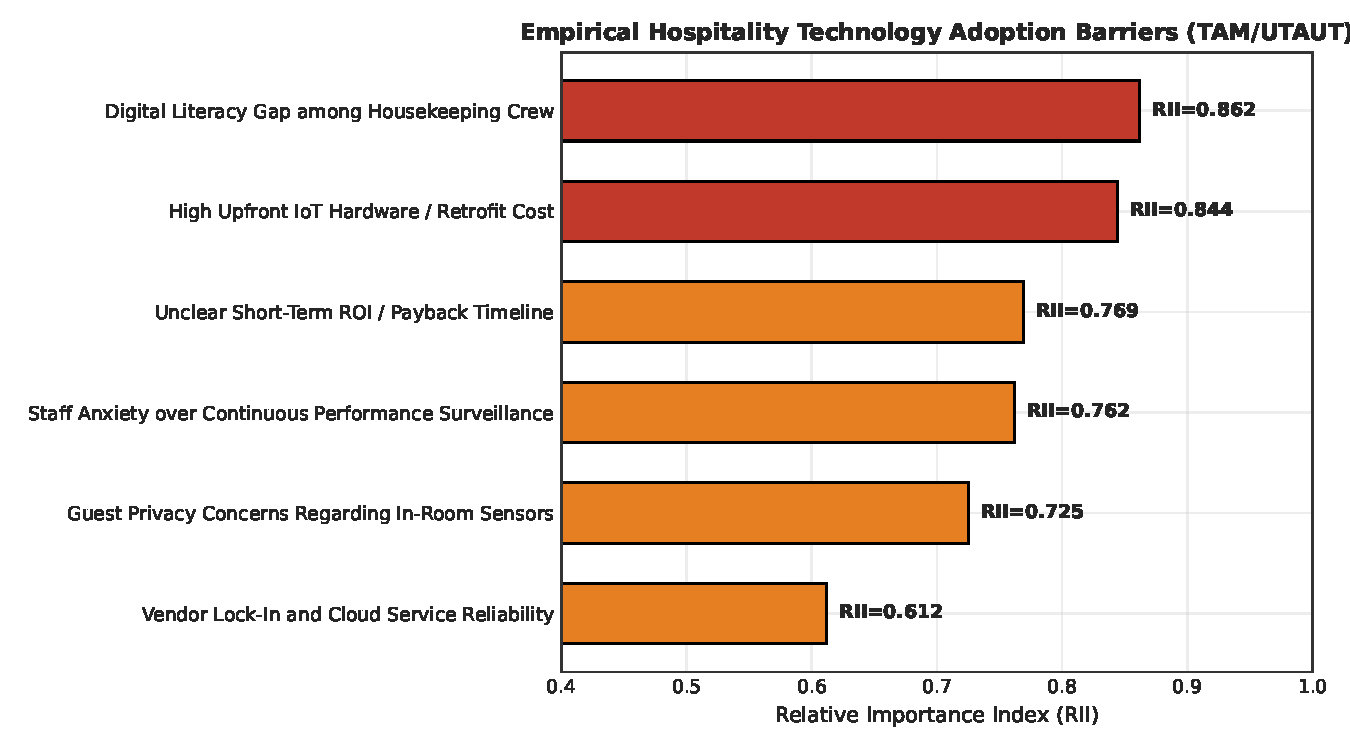
\includegraphics[width=0.85\textwidth,keepaspectratio]{figure6_tam_barrier_hierarchy.pdf}
\caption{Technology Acceptance Model (TAM) adoption governance: (a) Construct mean ratings across 32 hospitality leadership respondents; (b) Relative Importance Index (RII) barrier ranking across Criticality Tiers 1, 2, and 3.}
\label{fig:tam_hierarchy}
\end{figure}

As illustrated in Figure~\ref{fig:tam_hierarchy}(b), the digital literacy gap ($\text{RII} = 0.862$) and initial retrofit capital expenditure ($\text{RII} = 0.844$) constitute Tier 1 roadblocks. Table~\ref{tab:mitigation_framework} synthesizes actionable managerial strategies to resolve each empirical barrier.

\begin{table}[!htbp]
\centering
\small
\caption{Managerial mitigation framework addressing empirical technology adoption roadblocks.}
\label{tab:mitigation_framework}
\begin{tabularx}{\textwidth}{p{3.2cm} p{2.6cm} X}
\toprule
\textbf{Empirical Barrier} & \textbf{Theoretical Construct} & \textbf{Recommended Managerial Mitigation Strategy} \\
\midrule
\textbf{High Upfront IoT Cost} & Cost Constraints (CC) & Implement Hardware-as-a-Service (HaaS) subscription leasing to convert capital expenditure (CapEx) into operating expenditure (OpEx); initiate phased floor-by-floor rollouts. \\
\addlinespace
\textbf{Digital Literacy Gap} & Tech Resistance (TR) & Deploy icon-based, multilingual Progressive Web Apps (PWA) with color-coded room manifests; enforce zero-text workflows requiring under 15 minutes of employee training. \\
\addlinespace
\textbf{Surveillance Anxiety} & Tech Resistance (TR) & Decouple room completion tracking from punitive disciplinary actions; co-design operational interfaces with labor representatives; introduce gamified efficiency recognition. \\
\addlinespace
\textbf{Unclear Short-Term ROI} & Cost Constraints (CC) & Present verified 10,000-run Monte Carlo payback models (demonstrating 14--18 month breakeven) alongside quantified energy/water utility savings directly to property asset owners. \\
\addlinespace
\textbf{Guest Privacy Fears} & Privacy \& Trust (PT) & Install optical-blind passive infrared (PIR) and thermal motion sensors strictly; enforce a zero-camera/zero-microphone hardware policy prominently communicated on keycard jackets. \\
\bottomrule
\end{tabularx}
\end{table}

\section{CONCLUSION AND MANAGERIAL IMPLICATIONS}

This paper presented EcoHouse-AI, an integrated framework resolving the hospitality trilemma between guest satisfaction, environmental sustainability, and technology adoption barriers. By coupling aspect-based sentiment mining, unsupervised guest clustering, calibrated building energy physics, and TAM psychometrics, our findings demonstrate that:
\begin{enumerate}
    \item Domain-specific ABSA achieves 85.68\% classification accuracy and identifies promptness timing ($-0.2628$) as the primary driver of customer dissatisfaction.
    \item K-Means clustering segments guests into actionable operational personas, allowing properties to personalize linen and cleaning intensity.
    \item Smart eco-housekeeping reduces property electricity by 12.10\% (70,578 kWh/year) and water consumption by 4.32\% (476,824 L/year), abating 51.40 metric tonnes of $\text{CO}_2\text{e}$ in India and 28.04 metric tonnes in the United States annually for a standard 120-room property.
    \item Frontline digital literacy ($\text{RII} = 0.862$) and upfront CapEx ($\text{RII} = 0.844$) are the primary adoption bottlenecks, effectively mitigated via zero-text mobile interfaces, HaaS leasing, and optical-blind PIR sensors.
\end{enumerate}

\subsection{Managerial Takeaways}
Hospitality operators can transcend passive green marketing door cards by implementing digital guest profiling and automated room state coordination. Operational personalization delivers double-bottom-line benefits: protecting guest loyalty while achieving verifiable, audit-proof environmental carbon reductions.

\subsection{Limitations and Future Scope}
The environmental models in this study were calibrated against municipal commercial building disclosures (NYC LL84) and regional grid emission factors. Future research should deploy physical in-room IoT testbeds across diverse climatic zones, integrating real-time smart thermostat APIs and expanding TAM sample sizes across multinational chain portfolios.

\section*{DECLARATIONS}
\paragraph{Funding:} No external funding was received for conducting this research.
\paragraph{Conflicts of Interest:} The authors declare that they have no competing financial or personal interests.
\paragraph{Data Availability:} Public review and benchmarking data are accessible via cited repositories. Simulation code and survey instruments are available upon request.

\bibliographystyle{IEEEtran}
\begin{thebibliography}{30}

\bibitem{xiang2015}
Z.~Xiang, Z.~Schwartz, J.~H.~Gerdes, and M.~Uysal, ``What can big data and text analytics tell us about hotel guest experience and satisfaction?'' \emph{International Journal of Hospitality Management}, vol.~44, pp. 120--130, 2015. \url{https://doi.org/10.1016/j.ijhm.2014.10.013}

\bibitem{berezina2015}
K.~Berezina, A.~Bilgihan, C.~Cobanoglu, and F.~Okumus, ``Understanding satisfied and dissatisfied hotel customers: Text mining of online hotel reviews,'' \emph{Journal of Hospitality Marketing \& Management}, vol.~25, no.~1, pp. 1--24, 2015. \url{https://doi.org/10.1080/19368623.2015.983631}

\bibitem{min2015}
H.~Min, Y.~Lim, and V.~P.~Magnini, ``Factors affecting customer satisfaction in responses to complaints: Online hotel reviews,'' \emph{Cornell Hospitality Quarterly}, vol.~56, no.~2, pp. 224--235, 2015. \url{https://doi.org/10.1177/1938965514560014}

\bibitem{hutto2014}
C.~Hutto and E.~Gilbert, ``VADER: A parsimonious rule-based model for sentiment analysis of social media text,'' in \emph{Proceedings of the 8th International AAAI Conference on Weblogs and Social Media (ICWSM-14)}, 2014, pp. 216--225. \url{https://doi.org/10.1609/icwsm.v8i1.14550}

\bibitem{joachims1998}
T.~Joachims, ``Text categorization with Support Vector Machines: Learning with many relevant features,'' in \emph{Machine Learning: ECML-98}, ser. Lecture Notes in Computer Science, vol. 1398, Berlin: Springer, 1998, pp. 137--142. \url{https://doi.org/10.1007/bfb0026683}

\bibitem{rousseeuw1987}
P.~J.~Rousseeuw, ``Silhouettes: A graphical aid to the interpretation and validation of cluster analysis,'' \emph{Journal of Computational and Applied Mathematics}, vol.~20, pp. 53--65, 1987. \url{https://doi.org/10.1016/0377-0427(87)90125-7}

\bibitem{breiman2001}
L.~Breiman, ``Random forests,'' \emph{Machine Learning}, vol.~45, no.~1, pp. 5--32, 2001. \url{https://doi.org/10.1023/A:1010933404324}

\bibitem{bohdanowicz2006}
P.~Bohdanowicz, ``Environmental awareness and initiatives in the Swedish and Polish hotel sectors - attitudes, barriers and motivations,'' \emph{International Journal of Hospitality Management}, vol.~25, no.~4, pp. 662--682, 2006. \url{https://doi.org/10.1016/j.ijhm.2005.06.006}

\bibitem{chan2013}
E.~S.~W.~Chan, ``Gap analysis of green hotel marketing,'' \emph{International Journal of Contemporary Hospitality Management}, vol.~25, no.~7, pp. 1017--1048, 2013. \url{https://doi.org/10.1108/ijchm-09-2012-0156}

\bibitem{han2018}
H.~Han, J.~S.~Lee, H.~L.~T.~Trang, and W.~Kim, ``Water conservation and waste reduction management for increasing guest loyalty and green hotel practices,'' \emph{International Journal of Hospitality Management}, vol.~75, pp. 58--66, 2018. \url{https://doi.org/10.1016/j.ijhm.2018.03.012}

\bibitem{goldstein2008}
N.~J.~Goldstein, R.~B.~Cialdini, and V.~Griskevicius, ``A room with a viewpoint: Using social norms to motivate environmental conservation in hotels,'' \emph{Journal of Consumer Research}, vol.~35, no.~3, pp. 472--482, 2008. \url{https://doi.org/10.1086/586910}

\bibitem{wang2012}
J.~C.~Wang, ``A study on the energy performance of hotel buildings in Taiwan,'' \emph{Energy and Buildings}, vol.~49, pp. 268--275, 2012. \url{https://doi.org/10.1016/j.enbuild.2012.02.016}

\bibitem{bonilla2011}
M.~J.~Bonilla~Priego, J.~J.~Najera, and X.~Font, ``Environmental management decision-making in certified hotels,'' \emph{Journal of Sustainable Tourism}, vol.~19, no.~3, pp. 361--381, 2011. \url{https://doi.org/10.1080/09669582.2010.530350}

\bibitem{kang2021}
S.~Kang and S.~Nicholls, ``Determinants of willingness to pay to stay at green hotels,'' \emph{International Journal of Hospitality Management}, vol.~93, p. 102834, 2021. \url{https://doi.org/10.1016/j.ijhm.2020.102834}

\bibitem{verma2018}
V.~K.~Verma and B.~Chandra, ``An application of theory of planned behavior to predict young Indian consumers' green hotel visit intention,'' \emph{Journal of Cleaner Production}, vol.~172, pp. 1152--1162, 2018. \url{https://doi.org/10.1016/j.jclepro.2017.10.047}

\bibitem{hwang2019}
K.~Hwang and B.~Lee, ``Pride, mindfulness, public self-awareness, affective satisfaction, and customer citizenship behaviour among green hotel guests,'' \emph{International Journal of Hospitality Management}, vol.~83, pp. 169--179, 2019. \url{https://doi.org/10.1016/j.ijhm.2019.05.009}

\bibitem{sainaghi2019}
R.~Sainaghi, P.~Phillips, R.~Baggio, and A.~Mauri, ``Hotel performance: Rigor and relevant research topics,'' \emph{International Journal of Hospitality Management}, vol.~78, pp. 13--26, 2019. \url{https://doi.org/10.1016/j.ijhm.2018.11.008}

\bibitem{davis1989}
F.~D.~Davis, ``Perceived usefulness, perceived ease of use, and user acceptance of information technology,'' \emph{MIS Quarterly}, vol.~13, no.~3, pp. 319--340, 1989. \url{https://doi.org/10.2307/249008}

\bibitem{venkatesh2003}
V.~Venkatesh, M.~G.~Morris, G.~B.~Davis, and F.~D.~Davis, ``User acceptance of information technology: Toward a unified view,'' \emph{MIS Quarterly}, vol.~27, no.~3, pp. 425--478, 2003. \url{https://doi.org/10.2307/30036540}

\bibitem{venkatesh2012}
V.~Venkatesh, J.~Y.~Thong, and X.~Xu, ``Consumer acceptance and use of information technology: Extending the unified theory of acceptance and use of technology,'' \emph{MIS Quarterly}, vol.~36, no.~1, pp. 157--178, 2012. \url{https://doi.org/10.2307/41410412}

\bibitem{cronbach1951}
L.~J.~Cronbach, ``Coefficient alpha and the internal structure of tests,'' \emph{Psychometrika}, vol.~16, no.~3, pp. 297--334, 1951. \url{https://doi.org/10.1007/bf02310555}

\bibitem{tam2004}
C.~M.~Tam, V.~W.~Y.~Tam, and W.~S.~Tsui, ``Green construction assessment for environmental management in the construction industry of Hong Kong,'' \emph{International Journal of Project Management}, vol.~22, no.~7, pp. 563--571, 2004. \url{https://doi.org/10.1016/j.ijproman.2004.03.001}

\bibitem{khanra2021}
S.~Khanra, A.~Dhir, P.~Kaur, and R.~P.~Joseph, ``Factors influencing the adoption postponement of mobile payment services in the hospitality sector,'' \emph{Journal of Hospitality and Tourism Management}, vol.~46, pp. 26--39, 2021. \url{https://doi.org/10.1016/j.jhtm.2020.11.004}

\bibitem{ivanov2019}
S.~Ivanov and C.~Webster, ``Economic fundamentals of the use of robots, artificial intelligence, and service automation in travel, tourism, and hospitality,'' in \emph{Robots, Artificial Intelligence, and Service Automation in Travel, Tourism and Hospitality}, Bingley: Emerald Publishing, 2019, pp. 39--55. \url{https://doi.org/10.1108/978-1-78756-687-320191002}

\bibitem{buhalis1998}
D.~Buhalis and H.~Main, ``Information technology in peripheral small and medium hospitality enterprises: Strategic analysis and critical success factors,'' \emph{International Journal of Contemporary Hospitality Management}, vol.~10, no.~5, pp. 198--202, 1998. \url{https://doi.org/10.1108/09596119810227811}

\bibitem{krause2005}
N.~Krause, T.~Scherzer, and R.~Rugulies, ``Physical workload, work intensification, and prevalence of pain in low wage workers: Results from a participatory research project with hotel room cleaners in Las Vegas,'' \emph{American Journal of Industrial Medicine}, vol.~48, no.~5, pp. 326--337, 2005. \url{https://doi.org/10.1002/ajim.20221}

\bibitem{cea2024}
Central Electricity Authority, ``CO2 baseline database for the Indian power sector, User guide version 19.0,'' Ministry of Power, Government of India, New Delhi, Tech. Rep., 2024. [Online]. Available: \url{https://cea.nic.in/}

\bibitem{epa2024}
U.S. Environmental Protection Agency, ``Emissions \& generation resource integrated database (eGRID2022),'' Washington, DC, Tech. Rep., 2024. [Online]. Available: \url{https://www.epa.gov/egrid}

\bibitem{cornell2023}
Cornell Center for Hospitality Research, ``Cornell hotel sustainability benchmarking index (CHSB): Carbon, energy, and water,'' Cornell University, Ithaca, NY, Tech. Rep., 2023. [Online]. Available: \url{https://scholarship.sha.cornell.edu/chrpubs/}

\bibitem{nycll842023}
NYC Mayor's Office of Climate \& Environmental Justice, ``New York City Local Law 84 energy and water benchmarking report,'' New York, NY, Tech. Rep., 2023. [Online]. Available: \url{https://www.nyc.gov/site/sustainability/}

\end{thebibliography}

\end{document}
